\title{International Majorities Genuinely Support Global Redistributive and Climate Policies
} 

\begin{abstract}
  %

  We document majority support for policies entailing global redistribution and climate mitigation. Surveys on 40,680 respondents in 20 countries show strong stated support for a global carbon price funding equal cash transfers, called the ``Global Climate Scheme'' (GCS). Through our main surveys on 8,000 respondents in the U.S., France, Germany, Spain, and the UK, we test several hypotheses that could reconcile strong stated support with scarce occurrences in public debates. 
  Three quarters of Europeans and half of Americans support the GCS, even as they understand the policy's cost to them. Using different experiments, we show that the support for the GCS is sincere and that electoral candidates could win votes by endorsing it. More generally, we document widespread support for other globally redistributive policies, such as increased foreign aid or a wealth tax funding low-income countries. In sum, global policies are genuinely supported by majorities, even in wealthy, contributing countries.
  %
\end{abstract}

\tableofcontents

\onehalfspacing %

\begin{bibunit}

\section{Introduction}%

Major sustainability objectives could be achieved by global approaches to mitigating climate change and poverty involving transfers from high- to lower-income countries.\citep{budolfson_climate_2021,franks_mobilizing_2018,dennig_inequality_2015,soergel_combining_2021,bauer_quantification_2020,cramton_global_2017} 
Especially, global carbon pricing is widely regarded by economists as the benchmark climate policy, as it would efficiently correct the carbon emissions externality. A version of global carbon pricing as a system based upon tradable permits for carbon emissions is prominently discussed in environmental economics.\citep{grubb_greenhouse_1990,hoel_carbon_1991,agarwal_global_1991,bertram_tradeable_1992,baer_equity_2000,jamieson_climate_2001,blanchard_major_2021} It would work as follows: It implements a cap on carbon emissions to limit global warming below 2\textdegree{}C. The emission rights are auctioned each year to polluting firms and fund a global basic income, alleviating extreme poverty. The emission rights would be allocated 
equally among human adults, yielding redistribution from richer to poorer countries. It would combine long-term effectiveness, feasibility, equity, and simplicity.\citep{grubb_greenhouse_1990} We call this established approach to global carbon pricing the ``Global Climate Scheme'' (GCS).
While international negotiations have not yet led to ambitious globally redistributive policies, %
some recent prominent attempts are that the %
African Union \href{https://media.africaclimatesummit.org/NAIROBI+Declaration+FURTHER+edited+060923+EN+920AM.pdf}{calls for} a global carbon taxation regime, %
the UN \href{https://digitallibrary.un.org/record/4032838}{is setting up} a Framework Convention on International Tax Cooperation and  %
Brazil is proposing  
a global wealth tax at the G20. %

A key factor for implementing global policies has remained largely unaddressed: the support of citizens. Using a global survey on 40,680 respondents from 20 high- and middle-income countries, we reveal substantial support for global climate policies and, in addition, a global tax on the wealthiest aimed at financing low-income countries. Surprisingly, even in wealthy nations that would bear a significant burden, majorities of citizens express support for such globally redistributive policies. To better understand public support for global policies in high-income countries, the  main analysis of this article is conducted with surveys among 8,000 respondents from France, Germany, Spain, the UK, and the U.S. 
The focus of the main surveys is to study how respondents react to the key trade-off between the benefits and costs of globally redistributive climate policies. In our survey respondents are made aware of the cost that the GCS entails for their country's people, that is average Westerners would incur a net loss. Our main result is that the GCS is supported by three quarters of Europeans and more than half of Americans. 

Furthermore, we test the robustness of this conclusion by a wide variety of methods. First, we control for social desirability bias using a list experiment. We find no evidence that people exaggerate their support in the direct question. Second, to assess whether the support would diminish in a context with real stakes, we ask respondents whether they are willing to sign a petition in favor of the GCS, after informing them that the question results will be communicated to their head of state's office. The support is sustained in an environment that approaches real stakes. Third, we carry out conjoint analyses to neutralize experimenter demand and investigate the priority given to global policies compared to other types of policies. Conjoint analyses reveal that a political platform is more likely to be preferred if it contains the GCS or a global tax on millionaires, and that global policies rank high in the prioritization of policies. Our randomized experiments also show that a candidate would not lose vote intentions by endorsing the GCS, and might even gain up to 11 points in France. Fourth, an analysis of open-ended fields indicates that the appeal of the GCS comes from its international nature and its impacts on climate, more than on global poverty. %
To put our main finding in context, we also test other global policies and universalistic attitudes. Support is very strong for a global tax on millionaires, and the median respondent prefers to allocate 30\% of the revenues of such a tax to low-income countries. Majorities are willing to increase foreign aid, but only if some conditions are respected, such as making sure the aid is well spent and other high-income countries also increase their contribution. Questions on universalistic values, including a donation experiment, confirm the congruence of underlying values with the support for specific policies. Our diverse approaches also help understand what drives the support. For instance, the evidence indicates that one key reason why increasing foreign aid is not as popular as global policies lies in its unilateral nature.

Overall, our results %
point out to strong and genuine support for global climate and redistributive policies, as our experiments confirm the stated support found in direct questions. 
They contribute to a body of literature on attitudes toward climate policy, which confirms that climate policy is preferred at a global level,\citep{issp_international_2010,beiser-mcgrath_could_2019,sivonen_attitudes_2022,meilland_international_2023} where it is more effective and fair. 
While 3,354 economists supported a national carbon tax financing equal cash transfers in the \href{https://www.clcouncil.org/media/EconomistsStatement.pdf}{Wall Street Journal}, numerous surveys have shown that public support for such policy is mixed.\citep{douenne_yellow_2022,dechezlepretre_fighting_nodate,carattini_overcoming_2018,maestre-andres_perceived_2019,mildenberger_limited_2022,sommer_supporting_2022} Meanwhile, the GCS --- the global version of this policy --- is largely supported, despite higher costs in high-income countries. 
In the Discussion we offer potential explanations that could reconcile the strong support for global policies with their lack of prominence in the public debate. %
\paragraph{Literature} 

International surveys have shown widespread support for costly climate action.\citep{dechezlepretre_fighting_nodate,leiserowitz_international_2022} For instance, representative surveys in 125 countries covering 96\% of the world's greenhouse gas emissions show that 69\% of the global population express willingness to contribute 1\% of their income to fight global warming.\cite{andre_globally_2024} International surveys have also uncovered near consensus that ``present economic differences between rich and poor countries are too large'' (overall, 78\% agree and 5\% disagree) in each of 29 countries.\citep{issp_international_2019} 

Yet, few prior attitudinal surveys have examined global redistributive policies. 
A notable exception tests the support for six variants of a global carbon tax on samples in five countries, representative along gender and age.\cite{carattini_how_2019} For a given variant, the sample size is about 167 respondents per country. They find over 80\% support for any variant in India, between 50\% and 65\% in Australia, the UK and South Africa, and 43\% to 59\% in the U.S., depending on the variant. Notably, the support for a global carbon tax funding an equal cash transfer for each human is close to 50\% in high-income countries. %

Further evidence of the popularity of global redistribution is provided by the finding that 66\% of Americans support providing ``financial aid and technical support to developing countries that agree to limit their greenhouse gas emissions'';\cite{leiserowitz_public_2021} and 90\% of Germans want some degree of global redistribution.\cite{fehr_your_2022} 
Besides, in surveys conducted in Brazil, Germany, Japan, the UK and the U.S., support ranges from 55\% to 74\% for ``a global democracy including both a global government and a global parliament, directly elected by the world population, to recommend and implement policies on global issues'', and similar support is found in surveys over 17 countries.\cite{ghassim_who_2020,ghassim_who_2024} %

Appendix \ref{sec:literature} contains a broader literature review including further attitudinal surveys on global policies (\ref{subsubsec:literature_attitudes_policies}); prior work on attitudes toward climate burden sharing (Appendix \ref{subsubsec:literature_attitudes_burden_sharing}), attitudes toward foreign aid (Appendix \ref{subsubsec:literature_foreign_aid}), global carbon pricing (Appendix \ref{subsubsec:literature_pricing}), global redistribution (Appendix \ref{subsubsec:literature_redistribution}), basic income (Appendix \ref{subsubsec:literature_basic_income}), and global democracy (Appendix \ref{subsubsec:literature_democracy}).

\section{Results}

\subsection{Data}\label{subsec:data}

We use unanalysed questions from a global survey conducted in 2021 that involved 40,680 respondents from 20 countries, representing approximately 72\% of global CO$_\text{2}$ emissions. 
This survey (henceforth: global survey) serves as the basis for measuring stated support for various global policies worldwide. 
Detailed information about the data collection process, sample representativeness, and analysis of questions on national policies can be found in the companion paper.\cite{dechezlepretre_fighting_nodate}
To delve deeper into the sincerity and rationales behind support for the GCS and attitudes towards global policies, global redistribution, and universalistic values, we conducted further surveys  in 2023 (henceforth: main surveys). These surveys are based on a sample of 8,000 respondents from France, Germany, Spain, the UK, and the U.S. The European survey (\textit{Eu}) comprises 3,000 respondents, while the U.S. sample was collected in two separate waves: \textit{US1} with 3,000 respondents and \textit{US2} with 2,000 respondents. The survey questions in both the European and U.S. surveys are identical (see Figure \ref{fig:flow_simple}), except for an additional question in \textit{US2} that uses results from \textit{US1} to assess the bandwagon effect.
\begin{figure}[h!]
  \caption[Main surveys' structure]{Structure of main survey, cf. also Figure \ref{fig:flow_combined} for the treatment branches.}\label{fig:flow_simple}
  \makebox[\textwidth][c]{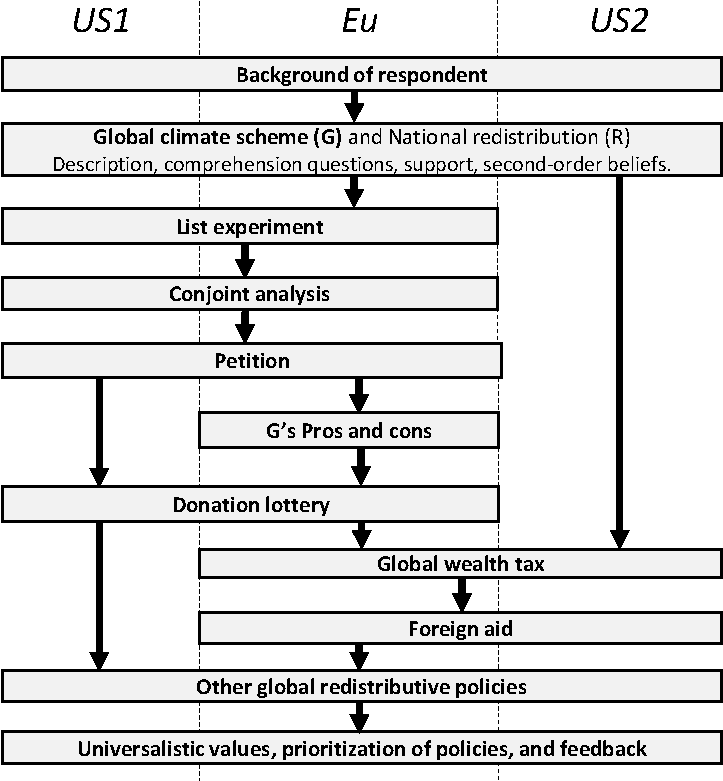
\includegraphics[width=.58\textwidth]{../questionnaire/survey_flow-simple.pdf}} 
\end{figure}
The main surveys ensured representativeness along key dimensions: gender, income, age, highest diploma, and degree of urbanization. The \textit{Eu} survey is also representative of its four countries in terms of population size, while the \textit{US1} and \textit{US2} surveys are representative in terms of region and ethnicity. 
Tables \ref{tab:representativeness_waves}-\ref{tab:representativeness_EU} detail how our samples match population frequencies. 
More detail on data collection is given in Section \nameref{sec:methods}. The questionnaires used in the surveys are provided in Appendices \ref{app:questionnaire_oecd} and \ref{app:questionnaire}.

\subsection{Global support}\label{subsubsec:global_support}

We find strong support for climate policies enacted at the global level when analysing the global survey (Figure \ref{fig:oecd}). %
When asked ``At which level(s) do you think public policies to tackle climate change need to be put in place?'', 70\% (in the U.S.) to 94\% (in Japan) choose the global level. The next most popular choice is the federal or continental level, favored by 52\% of Americans and less than half of European respondents. Local policies receive the least support. This preference for climate policies implemented at the global scale is in line with earlier contributions \cite{beiser-mcgrath_could_2019,bechtel_mass_2013,sivonen_attitudes_2022} %
and consistent with individuals' concerns for the fairness and effectiveness of such policies, which have been identified as two of the three key determinants of support, besides self-interest.\citep{klenert_making_2018,douenne_yellow_2022,dechezlepretre_fighting_nodate} It could also stem from conditional cooperation,\citep{barrett_self-enforcing_1994} even if previous studies suggest that the support for climate policies does not depend on climate action abroad \citep{aklin_prisoners_2020,tingley_conditional_2014}. %
\begin{figure}[h!]
  %
  \caption[Relative support for global climate policies]{Support for global climate policies.} 
  \makebox[\textwidth][c]{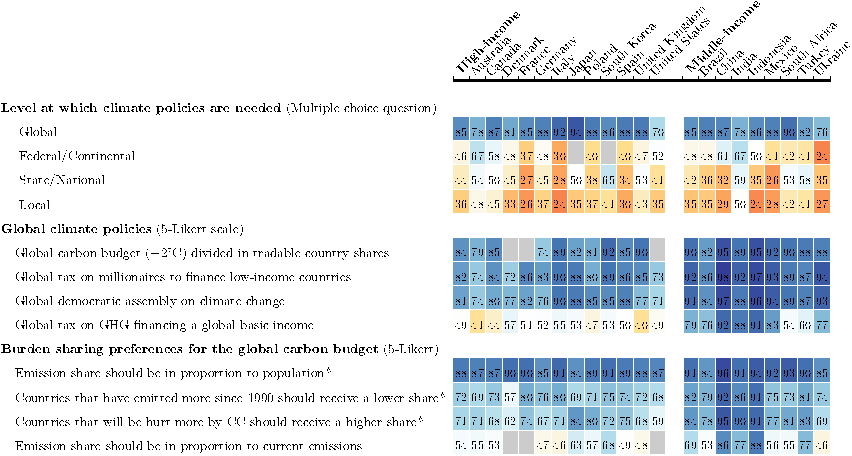
\includegraphics[width=1.2\textwidth]
  {../figures/OECD/Heatplot_global_tax_attitudes_share.pdf}}\label{fig:oecd} %
  {\footnotesize \\ $\quad$ \\ Note 1: The numbers represent \textit{relative} support, i.e. the share of \textit{Somewhat} or \textit{Strongly support} among non-\textit{indifferent} answers (in percent, $n$ = 40,680). The color blue denotes a relative majority. See Figure \ref{fig:oecd_absolute} for the absolute support. (Questions \ref{q:scale}-\ref{q:millionaire_tax}%
). \\ Note 2: *In Denmark, France and the U.S., the questions with an asterisk were asked differently, cf. Question \ref{q:burden_sharing_asterisk}. } 
\end{figure}

Among the four global climate policies examined, three policies garner high support across all countries (Figure \ref{fig:oecd}). These policies include a global democratic assembly on climate change, a global tax on millionaires to finance low-income countries contingent on their climate action, and a global carbon budget of +2\textdegree{}C divided among countries based on tradable shares (or ``global quota''), with the allocation of country shares unspecified (see wording in Appendix \ref{app:questionnaire_oecd}). 
The three policies garner a majority of absolute support (i.e., ``somewhat'' or ``strong'' support) in all countries (except in the U.S. for the global assembly, 48\% absolute support). In high-income countries, the global quota policy obtains 64\% absolute support and 84\% relative support (i.e., excluding ``indifferent'' answers). %

Following the support for the global quota, respondents are asked about their preferences for dividing the carbon budget among countries, as depicted in the third block of Figure \ref{fig:oecd}. Consistent with the existing literature (see Appendix \ref{subsubsec:literature_attitudes_burden_sharing}), an equal per capita allocation of emission rights emerges as the preferred burden-sharing principle, garnering absolute majority support in all countries and never below 84\% relative support. Taking into account historical responsibilities or vulnerability to climate damages is also popular, albeit with less consensus, while grandfathering (i.e., allocation of emission shares in proportion to current emissions) receives the least support in all countries.

A global carbon tax that funds a global basic income should produce the same distributional outcomes as a global tradable quota with equal per capita emission rights (to the extent that the carbon price is the same and provided that each country returns the revenues from emissions trading equally to its citizens). %
The support for the global carbon tax is also tested and its redistributive effects --  the average increase in expenditures along with the amount of the basic income -- are specified to the respondents explicitly  (see box below and Appendix \ref{app:questionnaire}, p.\pageref{subsec:questionnaire_GCS}). %
The support for the carbon tax is lower than for the quota, particularly in high-income countries, and there is no relative majority for the tax in Anglo-Saxon countries (consistently with the levels of support found in the only previous study that tested a global carbon tax\cite{carattini_how_2019}). %
Two possible reasons for this lower support are that distributive effects are specified explicitly in the case of the tax, and that people may prefer a quota, perhaps because they find it more effective than a tax to reduce emissions. The two reasons are consistent with the intermediate level of support for the GCS in the main survey, which is based on a global quota but where the question specifies explicitly the distributive effects. %

\subsection{Stated support for the Global Climate Scheme}\label{subsec:gcs_stated_support}

The main surveys (\textit{US1}, \textit{US2}, \textit{Eu}) include a comprehensive exploration of citizens' attitudes towards the GCS. We present to respondents a detailed description of the GCS and explain its distributive effects, including specific amounts at stake (as specified in the box below). Furthermore, we assess respondents' understanding of the GCS with incentivized questions to test their comprehension of the expected financial outcome for typical individuals in high-income countries (loss) and the poorest individuals globally (gain), followed by the provision of correct answers (Figures \ref{fig:understood_each}-\ref{fig:understood_score}). %

For comparison, %
the same approach is applied to a National Redistribution scheme (NR) targeting top incomes %
with the aim of financing cash transfers to all adults, %
calibrated to offset the monetary loss of the GCS for the median emitter in their country. We evaluate respondents' understanding that the richest would lose and the typical fellow citizens would gain from that policy. %
Subsequently, we summarize both schemes to enhance respondents' recall. Additionally, we present a final incentivized comprehension question and provide the expected answer that the combined GCS and NR would result in no net gain or loss for a typical fellow citizen. Finally, respondents are directly asked to express their support for the GCS and NR using a simple \textit{Yes}/\textit{No} question.

Our main result is that stated support for the GCS is 54\% in the U.S. and 76\% in Europe, while the support for NR is very similar: 56\% and 73\% respectively (Figures \ref{fig:support}, \ref{fig:support_binary}). 
Appendix \ref{app:determinants} examines the sociodemographic determinants of support for the GCS as well as the beliefs correlated with the support for a global tax on GHG financing a global basic income. The strongest correlates are political leaning, trust in the government and perceptions that climate policies are effective at reducing emissions or in one's self-interest. 

Finding majority support for the GCS runs counter to the conventional skepticism about the feasibility of global cooperation to mitigating climate change. %
This motivates the subsequent analysis of robustness and sincerity, novel to attitudinal surveys on instrument choice for environmental policy.  %

\begin{tcolorbox}\label{box:GCS}
  \paragraph{The Global Climate Scheme} The GCS consists of global emissions trading with emission rights being auctioned each year to polluting firms, and of a global basic income, funded by the auction revenues. Using the price and emissions trajectories from the report by Stern \& Stiglitz,\cite{stern_report_2017} and in particular a carbon price of \$90/tCO$_\text{2}$ in 2030, we estimate that the basic income would amount to \$30 per month for every human adult %
  (see details in Appendix \ref{app:gain_gcs}). %
  We describe the GCS to the respondents as a ``climate club'' and we specify its redistributive effects: The 700 million people with less than \$2/day [in Purchasing Power Parity] would be lifted out of extreme poverty, and fossil fuel price increases would cost the typical person in their country a specified amount (see Appendix \ref{subsec:questionnaire_GCS} for details). The monthly median net cost is \$85 in the U.S., \euro{}10 in France, \euro{}25 in Germany, \euro{}5 in Spain, £20 in the UK.
\end{tcolorbox}

\subsection{Stated support for global redistribution}\label{subsec:support_other}
We also assess support for a range of other international policies (Figure \ref{fig:support}) as well as unilateral foreign aid. %
\subsubsection{International policies}\label{subsubsec:support_other_global_policies} %

Most policies garner relative majority support in each country, with two exceptions: the ``cancellation of low-income countries' public debt'' and ``a maximum wealth limit'' for each individual (Figure \ref{fig:support}). %
The latter policy garners relative majority support in Europe but not in the U.S., despite the cap being set at \$10 billion in the U.S. compared to \euro{}/£100 million in Europe. Notably, climate-related policies enjoy significant popularity, with ``high-income countries funding renewable energy in low-income countries'' receiving absolute majority support across all surveyed countries. Additionally, relative support for loss and damages compensation, as approved in principle at the international climate negotiations in 2022 (``COP27''), ranges from 55\% (U.S.) to 81\% (Spain). %
Consistent with the results of the global survey, 
a ``tax on millionaires of all countries to finance low-income countries'' garners relative support of over 69\% in each country, only 5 p.p. lower than a national millionaires tax overall. In random subsamples, we inquire about respondents' preferences regarding the redistribution of revenues from a global tax on individual wealth exceeding \$5 million, after providing information on the revenue raised by such a tax in their country compared to low-income countries. 
We ask certain respondents ($n$ = 1,283) what percentage of the global tax revenues should be pooled to finance low-income countries. In each country, at least 88\% of respondents indicate a positive amount, with an average of one-third %
(Figure \ref{fig:global_share_mean}). To other respondents ($n$ = 1,233), we inquire whether they would prefer each country to retain all the revenues it collects or that half of the revenues be pooled to finance low-income countries. Approximately half of the respondents opt to allocate half of the tax revenues to low-income countries, consistently with the other variant of the question.
\begin{figure}
  %
  \caption[Relative support for other global policies]{Support for various global policies. (\textit{relative support}: percentage of \textit{somewhat} or \textit{strong support}, after excluding \textit{indifferent} answers; *except for GCS: percentage of \textit{Yes} in a \textit{Yes}/\textit{No} question). (p. \pageref{subsec:questionnaire_GCS}, Questions \ref{q:gcs_support}, \ref{q:climate_policies} and \ref{q:other_policies}; See Figure \ref{fig:support_likert_positive} for the absolute support.)%
  }
  \makebox[\textwidth][c]{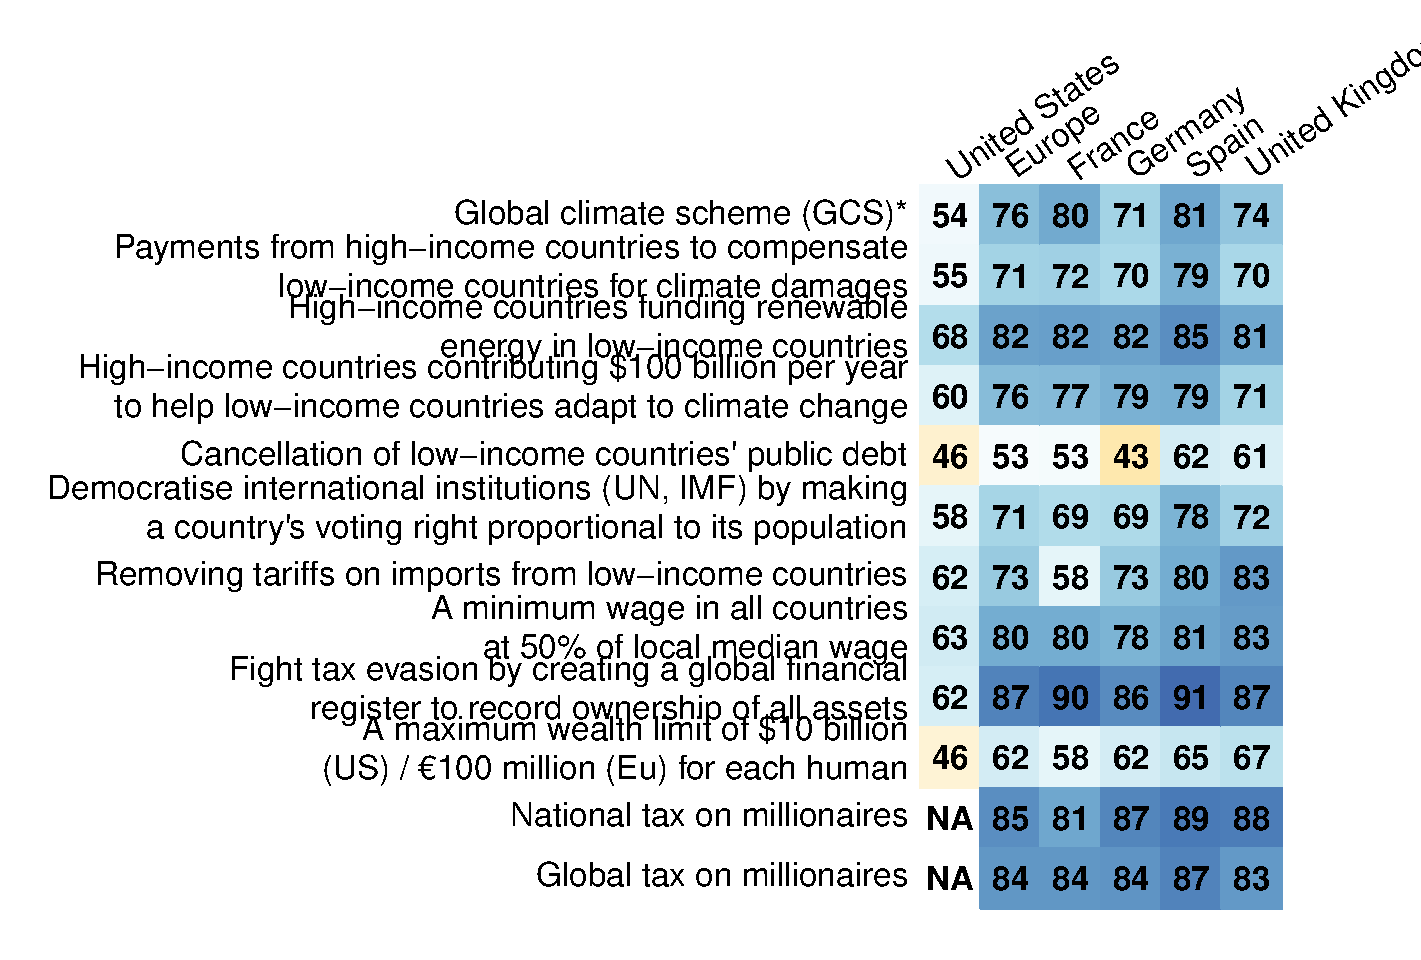
\includegraphics[width=\textwidth]{../figures/country_comparison/support_likert_gcs_share.pdf}}\label{fig:support}
\end{figure} 

\subsubsection{Foreign aid}\label{subsubsec:support_foreign_aid} %

In addition, we provide respondents with information about the actual amount ``spent on foreign aid to reduce poverty in low-income countries'' relative to their country's government spending and GDP. Less than 16\% of respondents state that their country's foreign aid should be reduced, while 62\% express support for increasing it, including 17\% who support an unconditional increase (Figure \ref{fig:foreign_aid_raise_support}). Among the 45\% who think aid should be increased under certain conditions, we subsequently ask them to specify the conditions they deem necessary (Figure \ref{fig:foreign_aid_condition}). The three most commonly selected conditions are that: ``we can be sure the aid reaches people in need and money is not diverted'' (73\% chose this condition), ``recipient countries comply with climate targets and human rights'' (67\%), and ``other high-income countries also increase their foreign aid'' (48\%). %
On the other hand, respondents who do not wish to increase their country's foreign aid primarily justify their view by prioritizing the well-being of their fellow citizens or by perceiving each country as responsible for its own fate (Figure \ref{fig:foreign_aid_no}). In response to an open-ended question regarding measures high-income countries should take to fight extreme poverty, a large majority of Americans expressed that more help is needed (Figure \ref{fig:poverty_field}). The most commonly suggested form of aid is financial support, closely followed by investments in education. 

We also inquire about the perceived amount of foreign aid. Consistent with prior research (see Appendix \ref{subsubsec:literature_foreign_aid}), most people overestimate the actual amount of foreign aid (Figure \ref{fig:foreign_aid_belief}). We then elicit respondents' preferred amount of foreign aid, after randomly presenting them with either the actual amount or no information. Most of the respondents who learn the actual amount choose a bracket at least as high as the actual one, and most of those without the information choose a bracket at least as high as the perceived one (Figures \ref{fig:foreign_aid_amount}--\ref{fig:foreign_aid_preferred_info}). Finally, we ask a last question to the respondents who received the information. To those who prefer an increase of foreign aid, we ask how they would finance it: by far, the preferred source of funding is higher taxes on the wealthiest (Figure \ref{fig:foreign_aid_raise_how}). To those who prefer a reduction, we ask how they would use the funds becoming available: %
In every country, more people choose higher spending on education or healthcare rather than lower taxes (Figure \ref{fig:foreign_aid_reduce_how}). 

\subsection{Robustness and sincerity of support for the GCS}\label{subsec:robustness_sincerity}
We use several methods to assess the sincerity of the support for the GCS: a list experiment, a real-stake petition, conjoint analyses, and the prioritization of policies. All methods suggest that the support is either completely sincere, or the share of insincere answers is limited. 

\subsubsection{List experiment}\label{subsubsec:list_exp} %

By asking \textit{how many} policies within a list respondents support and varying the list among respondents, a list experiment allows identifying the tacit support for a policy of interest. 
For example, say a first subsample faces the list of policies A, B, and C, while a second subsamples faces the list A, B, C, and GCS. We do not need to know which policies each respondent support to estimate the average (tacit) support for the GCS, we simply need to compute the difference in the average number of supported policies between the two random subsamples.\citep{imai_multivariate_2011} 
In our case, as shown in Table \ref{tab:list_exp}, the tacit support for the GCS measured through the list experiment is not significantly lower than the direct stated support. %
Hence, we do not find a social desirability bias in our study.

\subsubsection{Petition}\label{subsubsec:petition} %

We ask respondents whether they are willing to sign a petition in support of either the GCS or NR policy. We inform them that the petition results will be sent to the head of state's office, highlighting the proportion of fellow citizens endorsing the respective scheme. Even when framed as a petition that might have real stakes, both policies continue to receive majority support. In the U.S., we find no significant difference between the support in the %
petitions and the simple questions (GCS: $p=.30$; NR: $p=.76$). %
In Europe, the petition leads to a comparable lower support for both the GCS (7 p.p., $p=10^{-5}$) and NR (4 p.p., $p = .008$). While some European respondents are unwilling to sign a petition for policies they are expected to support, this phenomenon is not specific to the GCS, and the overall willingness to sign a %
petition remains strong, with 69\% expressing support for the GCS and 67\% for NR.

\subsubsection{Conjoint analyses}\label{subsubsec:conjoint} %

In order to assess the public support for the GCS in conjunction with other policies, we conduct a series of conjoint analyses. We ask respondents to make five choices between pairs of political platforms. Each choice is meant at testing a different hypothesis on the support for the GCS in relation to other policies or voting.

The first conjoint analysis suggests that the GCS is supported independently of being complemented by the National Redistribution Scheme and a national climate policy (C). %
The second analysis indicates majority support for the GCS and for C, which are seen as neither complement nor substitute (see \nameref{sec:methods}). A minor share of respondents like a national climate policy and dislike a global one, but as many people prefer a global rather than a national policy; and there is no evidence that implementing NR would increase the support for the GCS.
In the third analysis, we present two random branches of the sample with hypothetical progressive and conservative platforms that differ only by the presence (or not) of the GCS in the progressive platform. Table \ref{tab:conjoint_c} shows that a progressive candidate would not significantly lose voting share by endorsing the GCS in any country, and may even gain 11 p.p. ($p = .005$) in voting intention in France. %
Our last two analyses make respondents choose between two random platforms. In Europe, respondents are prompted to imagine that a left or center-left coalition will win the next election and asked what platform they would prefer that coalition to have campaigned on. In the U.S., the question is framed as a hypothetical duel in a Democratic primary, and asked only to non-Republicans ($n$ = 2,218), i.e. the respondents who declare as political affiliation \textit{Democrat}, \textit{Independent}, \textit{Non-Affiliated} or \textit{Other}. 

In the fourth analysis, a policy (or an absence of policy) is randomly drawn for each platform in each of five categories: \textit{economic issues}, \textit{societal issues}, \textit{climate policy}, \textit{tax system}, \textit{foreign policy} (Figure \ref{fig:ca_r}). 
In the UK, Germany, and France, a platform is about 9 to 13 p.p. more likely to be preferred if it includes the GCS rather than no foreign policy. %
This effect is between 1 and 4 p.p. and no longer significant in the U.S. (among non-Republicans) and in Spain. Moreover, a platform that includes a global tax on millionaires rather than no foreign policy is 5 to 13 p.p. more likely to be preferred in all countries (the effect is significant and at least 9 p.p. in all countries but Spain). 
Similarly, a global democratic assembly on climate change has a significant effect of 8 to 12 p.p. in the U.S. (among non-Republicans), Germany, and France. 
These effects are large, and not far from the effects of the policies most influential on the platforms, which range between 15 and 18 p.p. in most countries (27 p.p. in Spain), and all relate to improved public services (in particular healthcare, housing, and education).
 
The fifth analysis draws random platforms similarly, except that candidate A's platform always contains the GCS while B's includes no foreign policy. In this case, A is chosen by 60\% of Europeans %
and 58\% of non-Republican Americans (Figure \ref{fig:conjoint_left_ag_b}). %

Overall, taking the U.S. as an example, our conjoint analyses indicate that a candidate at the Democratic primary would have more chances to obtain the nomination by endorsing the GCS, and this endorsement would not penalize her or him at the presidential election. 
This result relates to the finding that 12\% of Germans shift their voting intention from SPD and CDU/CSU to the Greens and the Left when they are told that the latter parties support global democracy.\citep{ghassim_who_2020}
\subsubsection{Prioritization}\label{subsubsec:prioritization} %

Towards the end of the survey, we ask respondents to allocate 100 points among six randomly selected policies from the previous conjoint analyses, using sliders. The instruction was to distribute the points based on their level of support, with a higher allocation indicating greater support for a policy. %
As a result, the average support across policies is 16.67 points. %
In each country, the GCS ranks in the middle of all policies or above, with an average number of points from 15.4 in the U.S. to 22.9 in Germany.%

Interestingly, in Germany, the most prioritized policy is the global tax on millionaires, while the GCS is the second most prioritized policy. The global tax on millionaires consistently ranks no lower than fifth position (out of 15 or 17 policies) in every country, garnering an average of 18.3 points in Spain to 22.9 points in Germany.

  
\subsubsection{Pros and Cons}\label{subsubsec:pros_cons}

We survey respondents to gather their perspectives on the pros and cons of the GCS, randomly utilizing an open-ended or a closed question. In the closed question format, respondents tend to consider every argument as important in determining their support or opposition to the GCS (see Figure \ref{fig:gcs_important}). 

The open-ended question provides more insights into what people associate with the GCS when prompted to think about it. %
Analyzing keywords in the responses (automatically translated into English), the most frequently mentioned topics are the international aspect and the environment, each appearing in approximately one-quarter of the answers (see Figure \ref{fig:gcs_field_contains}). This is followed by discussions on the effects of the GCS on poverty and prices, each mentioned by about one-tenth of the respondents. We also manually classified each answer into different categories (see Figure \ref{fig:gcs_field}). This exercise confirms the findings from the automatic search: the environmental benefit of the GCS is the most commonly discussed topic, while obstacles to implementation or agreement on the proposal are relatively infrequently mentioned.%

In the \textit{US2} survey, we divided the sample into four random branches. Two branches were presented the pros and cons questions (either in open or closed format) \textit{before} being asked about their support for the GCS or NR. Another branch received information on the actual level of support for the GCS and NR (estimated in \textit{US1}, see box p. \pageref{subsec:second_order_beliefs}), %
and one control group received none of these treatments. %
The objective of the ``pros and cons treatment'' was to mimic a ``campaign effect'', which refers to the shift in opinion resulting from media coverage of the proposal.\citep{anderson_can_2023} To conservatively estimate the effect of a (potentially negative) campaign, we intentionally included more cons (6) than pros (3). Interestingly, the support for the GCS decreased by 11 p.p. after respondents viewed a list of its pros and cons. %
Notably, the support also decreased by 7 p.p. after respondents were asked to consider the pros and cons in an open-ended question. Despite some significant effects of pondering the pros and cons, approximately half of the Americans express support for the GCS across all treatment branches (see Table \ref{tab:branch_gcs}). Although support remains significant, %
these results suggest that the public success of the GCS would be sensitive to the content of the debate about it, and oriented by the discourse adopted by interest groups. %
\begin{tcolorbox}\label{subsec:second_order_beliefs}
  \paragraph{Second-order Beliefs}
To explain the strong support for the GCS despite its absence from political platforms and public debate, we hypothesized pluralistic ignorance, i.e. that the public and policymakers mistakenly perceive the GCS as unpopular. As a result, individuals might conceal their support for such globally redistributive policy, believing that advocating for it would be futile. 

In the case of Americans, their beliefs about the level of support for the GCS are relatively accurate (Figure \ref{fig:belief}). The mean perceived support is 52\% (with quartiles of 36\%, 52\%, and 68\%), which closely aligns with the actual support of 54\%. Europeans, on the other hand, underestimate the support by 17 p.p. Nonetheless, 65\% of them correctly estimate that the GCS garners majority support, and the mean perceived support is 59\% (and quartiles of 43\%, 61\%, and 74\%), compared to the actual support of 76\%. %
Second-order beliefs are equally accurate for NR in the U.S. and similarly underestimated in Europe. %
Finally, consistent with Americans accurately perceiving the levels of support for the GCS or NR, providing information on the actual level had no significant effect on their support in the \textit{US2} survey. %
\end{tcolorbox}

\subsection{Universalistic values}\label{subsec:universalistic}

We elicit underlying values, to test whether broad values are consistent with people's support for specific policies. %
When we ask respondents which group they defend when they vote, %
20\% choose ``sentient beings (humans and animals),'' 22\% choose ``humans,'' 33\% select their ``fellow citizens'' (or ``Europeans''), 15\% choose ``My family and myself,'' and the remaining 10\% choose another group (mainly ``My State or region'' or ``People sharing my culture or religion''). 
Notably, a majority of left-wing voters choose \textit{humans} or \textit{sentient beings}. 

Answers to this and other broad value questions are consistent with half of Americans and three quarters of Europeans supporting global policies like the GCS: people are almost as much willing to make a donation to poor Africans than to poor fellow citizens in a lottery experiment, most respondents find that global issues are among the biggest problems, and most respondents wish that their diplomats take into account global justice (see \nameref{sec:methods} for details).
\section{Discussion} %

In our analysis, we have uncovered strong and genuine support for global redistributive policies. One limitation to this finding, inherent to any inquiry into hypothetical policies, is that the support might change once global policies are discussed in the public debate (as explored in the paragraph on \textit{Pros and Cons}). 

We conclude by providing hypotheses to reconcile the scarcity of global policies in the public debate with our findings that they would be widely accepted. %
The first two are variations of pluralistic ignorance, and the last three represent complementary explanations. 

First, there may be pluralistic ignorance \textit{among policymakers} regarding universalistic values, support for the GCS, or the electoral advantage of endorsing it. 
Second, people or policymakers may believe that globally redistributive policies are politically infeasible in some key (potentially foreign) countries like the U.S. %
Third, political discourse centrally happens at the national level, shaped by national media and institutions such as voting. 
National framing by political voices may create biases and suppress universalistic values. %
Fourth, many individuals, including policymakers, may perceive global redistributive policies as ill-defined or technically infeasible, ultimately dismissing them as unrealistic. In particular, policymakers may have insider information about the technical feasibility of such policies. Alternatively, the perception of unrealism may stem from an unawareness of specific proposals. %
Fifth, just as policy is disproportionately influenced by the economic elites,\citep{gilens_testing_2014,persson_rich_2023} public debate may be shaped by the wealthiest, who have vested interests in preventing global redistribution.

Confirmation of any of these hypotheses would lead to a common conclusion: there exists substantial public support for global policies addressing climate change and global inequality, even in high-income countries. %
Uncovering evidence to support the above hypotheses could %
draw attention to global policies in the public debate and contribute to their increased prominence. %
  \begin{small} %
\section*{\normalsize Methods}\label{sec:methods} %
\addcontentsline{toc}{section}{\nameref{sec:methods}}

\paragraph{\small Pre-registration.}
The project is approved by Economics \& Business Ethics Committee (EBEC) at the University of Amsterdam (EB-1113) and %
was preregistered in the Open Science Foundation registry (\href{https://osf.io/fy6gd}{osf.io/fy6gd}). The study did not deviate from the registration: the questionnaires and the hypotheses tests used are the same as the ones \href{https://osf.io/2b6vq}{given \textit{ex ante}}. Informed consent was obtained from all respondents, randomized treatment branches were unkown to the respondents, and our research complies with all relevant ethical regulations. Respondents were compensated with gift certificates for a value of \euro{}1 per interview. No statistical methods were used to pre-determine sample sizes but our sample sizes match those reported in similar publications.\citep{dechezlepretre_fighting_nodate,issp_international_2010,beiser-mcgrath_could_2019,sivonen_attitudes_2022,douenne_yellow_2022}

\paragraph{\small Data collection.} %

The paper utilizes two sets of surveys: the \textit{global} survey and the \textit{m} surveys. The \textit{main} surveys consist of two U.S. surveys, \textit{US1} and \textit{US2}, and one European survey, \textit{Eu}. The \textit{global} survey was conducted from March 2021 to March 2022 on 40,680 respondents from 20 countries (with 1,465 to 2,488 respondents per country). \textit{US1} collected responses from 3,000 respondents between January and March 2023, while \textit{US2} gathered data from 2,000 respondents between March and April 2023. \textit{Eu} included 3,000 respondents and was conducted from February to March 2023. We used the survey companies \emph{Dynata} and \emph{Respondi}. To ensure representative samples, we employed stratified quotas based on gender, age (5 brackets), income (4), region (4), education level (3), and ethnicity (3) for the U.S. We also incorporated survey weights throughout the analysis to account for any remaining imbalances. These weights were constructed using the quota variables as well as the degree of urbanity, and trimmed between 0.25 and 4. Stratified quotas followed by reweighting is the usual method to reduce selection bias from opt-in online panels, when better sampling methods (such as compulsory participation of random dwellings) are unavailable.\cite{scherpenzeel_how_2010} By applying weights, the results are fully representative of the respective countries along the above mentioned dimensions. %
Results at the European level apply different weights which ensure  representativeness of the combined four European countries. Appendix \ref{app:representativeness} shows how our samples compare to actual population frequencies. Our samples match the actual frequencies well, except for some imbalance in the U.S. vote (which does not affect our results, as shown by the results reweighted by vote in the \textit{Support for the GCS} section below). 
Appendix \ref{app:balance} shows that the treatment branches are balanced. Appendix \ref{app:placebo} runs placebo tests of the effects of each treatment on unrelated outcomes. We do not find effects of earlier treatments on unrelated outcomes arriving later in the survey. Appendix \ref{app:extended} shows that our results are unchanged when including inattentive respondents.
\paragraph{\small Data quality.} %
The median duration is 28 minutes for the \textit{global} survey, 14 min for \textit{US1}, 11 min for \textit{US2}, and 20 min for \textit{Eu}. To ensure the best possible data quality, we exclude respondents who fail an attention test or rush through the survey (i.e., answer in less than 11.5 minutes in the \textit{global} survey, 4 minutes in \textit{US1} or \textit{US2}, 6 minutes in \textit{Eu}). %
At the end of the survey, we ask whether respondents thought that our survey was politically biased and offer to provide some feedback. 67\% of the respondents found the survey unbiased. 25\% found it left-wing biased, and 8\% found it right-wing biased.

\paragraph{\small Questionnaires and raw results.} %
The raw results are reported in Appendix \ref{app:raw_results} while the surveys' structures and questionnaires are given in Appendices \ref{app:questionnaire_oecd} and \ref{app:questionnaire}. Details on the \textit{global} survey can be found in the Appendix of the companion paper.\citep{dechezlepretre_fighting_nodate} Country-specific raw results are also available as supplementary material files:  \href{https://github.com/bixiou/international_attitudes_toward_global_policies/raw/main/paper/app_desc_stats_US.pdf}{US}, \href{https://github.com/bixiou/international_attitudes_toward_global_policies/raw/main/paper/app_desc_stats_EU.pdf}{EU}, \href{https://github.com/bixiou/international_attitudes_toward_global_policies/raw/main/paper/app_desc_stats_FR.pdf}{FR}, \href{https://github.com/bixiou/international_attitudes_toward_global_policies/raw/main/paper/app_desc_stats_DE.pdf}{DE}, \href{https://github.com/bixiou/international_attitudes_toward_global_policies/raw/main/paper/app_desc_stats_ES.pdf}{ES}, \href{https://github.com/bixiou/international_attitudes_toward_global_policies/raw/main/paper/app_desc_stats_UK.pdf}{UK}. %
\paragraph{\small Incentives.} %
To encourage accurate and truthful responses, several questions of the main surveys use incentives. For each of the three comprehension questions that follow the policy descriptions, we randomly select and reward three respondents who provide correct answers with a \$50 gift certificate. Similarly, for questions involving estimating support shares for the GCS and NR, three respondents with the closest guesses to the actual values receive a \$50 gift certificate. In the donation lottery question, we randomly select one respondent and split the \$100 prize between the NGO GiveDirectly and the winner according to the winner's choice. In total, our incentives scheme distributes gift certificates (and donations) for a value of \$850. Finally, respondents have an incentive to answer truthfully to the petition question, as they are aware that the results for that question (the share of respondents supporting the policy) will be transmitted to their head of state's office.
\paragraph{\small Absolute vs. relative support.}
In most questions, support or opposition for a policy is asked using a 5-Likert scale, with compulsory response and \textit{Indifferent} as the middle option. We call \textit{absolute support} the share of \textit{Somewhat} or \textit{Strong support}. We generally favor the notion of \textit{relative support}, which reports the share of support after excluding \textit{Indifferent} answers. Indeed, the \textit{relative support} is better suited to assess whether there are more people in favor vs. against a policy.

\paragraph{\small Support for the GCS.} 
The 95\% confidence intervals are $[52.4\%, 55.9\%]$ in the U.S. and $[74.2\%, 77.2\%]$ in Europe. The average support is computed with survey weights, employing weights based on quota variables, which exclude vote. Another method to reweigh the raw results involves running a regression of the support for the GCS on sociodemographic characteristics (including vote) and multiplying each coefficient by the population frequencies. This alternative approach yields similar figures: 76\% in Europe and 52\% or 53\% in the U.S. (depending on whether individuals who did not disclose their vote are classified as non-voters or excluded). Notably, the average support among voters is 54\% in the U.S., with 74\% support among Biden voters vs. 26\% among Trump voters (see Figure \ref{fig:main_by_vote}).

Though the level of support for the GCS is significantly lower in swing States (at 51\%) that are key to win U.S. elections, the electoral effect of endorsing the GCS remains non-significantly different from zero (at +1.2 p.p.) in these States. Note that we define swing states as the 8 states with less than 5 p.p. margin of victory in the 2020 election (MI, NV, PA, WI, AZ, GA, NC, FL). The results are unchanged if we use the 3 p.p. threshold (that excludes FL) instead. 

\paragraph{\small List experiment.} %
List experiments have been used to reveal social desirability bias, silencing either racism in the Southern U.S.\citep{kuklinski_racial_1997} or opposition to the invasion of Ukraine in Russia.\citep{chapkovski_solid_2022} %
In our case, the question reads: ``Beware, this question is quite unusual. Among the policies below, \textbf{how many} do you support?'' The list of policies randomly varies across respondents, and includes a subset of GCS, NR (National Redistribution scheme), C (``Coal exit'' in the U.S., ``Thermal insulation plan'' in Europe) and O (``Marriage only for opposite-sex couples in the U.S.'', ``Death penalty for major crimes'' in Europe). There are four branches: GCS/NR/C/O; GCS/C/O; NR/C/O; C/O. To estimate the tacit average support for the GCS and NR, we regress the number of supported policies on indicators that the list includes GCS and NR.
We utilize the difference-in-means estimator, and confidence intervals are computed using Monte Carlo simulation with the R package \textit{list}.\citep{imai_multivariate_2011}

\paragraph{\small Petition.}
The respondent is randomly assigned a branch where the petition relates to the GCS or the National Redistribution scheme. The question reads: ``Would you be willing to sign a petition for the [Global climate / National redistribution] scheme? \\ As soon as the survey is complete, we will send the results to [the U.S. President's office], informing him what share of [American] people are willing to endorse the [Global climate / National redistribution] scheme. (You will NOT be asked to sign, only your answer here is required and remains anonymous.)''. 

Paired weighted \textit{t}-tests are conducted to test the equality in support for a policy among respondents who were questioned about the policy in the petition.

\paragraph{\small Conjoint analyses.}
The first conjoint analysis suggests that the GCS is supported independently of being complemented by the National Redistribution Scheme and a national climate policy (``Coal exit'' in the U.S., ``Thermal insulation plan'' in Europe, denoted C). Indeed, 54\% of %
U.S. respondents and 74\% of %
European ones prefer the combination of C, NR and the GCS to the combination of C and NR alone, indicating similar support for the GCS conditional on NR and C than for the GCS alone (Figure \ref{fig:conjoint}). 

In the second conjoint analysis, results from the first branch show that the support for the GCS conditional on NR, at 55\% in the U.S. ($n$ = 757) and 77\% in Europe ($n$ = 746), is not significantly different from the support for the GCS alone. This suggests that rejection of the GCS is not driven by the cost of the policy on oneself. The second branch shows that the support for C conditional on NR is somewhat higher, at 62\% in the U.S. ($n$ = 751) and 84\% in Europe ($n$ = 747). However, the third one shows no significant preference for C compared to GCS (both conditional on NR), neither in Europe, where GCS is preferred by 52\% ($n$ = 741) nor in the U.S., where C is preferred by 53\% ($n$ = 721). The fourth branch shows that 55\% in the U.S. ($n$ = 771) and 77\% in Europe ($n$ = 766) prefer the combination of C, NR and the GCS to NR alone.

The effects reported in the fourth analysis are the Average Marginal Component Effects.\cite{hainmueller_causal_2014} The policies studied are progressive policies prominent in the country. Except for the category \textit{foreign policy}, which features the GCS 42\% of the time, they are drawn uniformly.

\paragraph{\small Prioritization.}
The prioritization allows inferring individual-level preferences for one policy over another, including in their intensity. This somewhat differs from a conjoint analysis, which only allows inferring individual-level preferences for one platform over another or collective-level preferences for one policy over another. Also, by comparing platforms, conjoint analyses may be subject to interaction effects between policies of a platform (which can be seen as complementary, substitute, or antagonistic) while the prioritization frames the policies as independent.

This question sheds light on a potential discrepancy between the policy priorities of the public and those enacted by legislators. For instance, while the European Union and California have enacted plans to phase out new combustion-engine cars by 2035, the proposal to ``ban the sale of new combustion-engine cars by 2030'' emerged as one of the three least prioritized policies in each country, with an average allocation of 7.8 points in France to 11.4 points in the UK.

\paragraph{\small Open-ended question on the GCS.}
Around one in four respondents explicitly cites pros or cons. Few individuals explicitly express support or opposition, and misunderstandings are rare. Only 11\% of the responses are empty or express a lack of opinion, though one-quarter are unclassifiable due to the rarity, nonsensical nature, or irrelevance of the conveyed idea.

\paragraph{\small Pros and cons.}
In the closed question, the least important aspect was the negative impact on their household, with 60\% in Europe ($n$=1,505) and 75\% in the U.S. ($n$=493) finding it important. The most important elements differ between Europe and the U.S. In Europe, the key factors are the GCS's potential to limit climate change and reduce poverty in low-income countries, both deemed important by 85\% of respondents. In the U.S., having sufficient information about the scheme ranks highest at 89\%, followed by its potential to foster global cooperation at 82\%. 

Surprisingly, the support for National Redistribution also decreased by 7 p.p. following the closed question about the GCS. This suggests that some individuals may lack attention and confuse the two policies, or that contemplating the pros and cons alters the mood of some people, moving them away from their initial positive impression.

\paragraph{\small Universalistic values}
When asked what their country's diplomats should defend in international climate negotiations, only 11\% prefer their country's ``interests, even if it goes against global justice.'' In contrast, 30\% prefer global justice (with or without consideration of national interests), and the bulk of respondents (38\%) prefer their country's ``interests, to the extent it respects global justice.''

Furthermore, when we ask respondents to assess the extent to which climate change, global poverty, and inequality in their country are issues, climate change is generally viewed as the most significant problem %
(with a mean score of 0.59 after recoding answers between -2 and 2). This is followed by global poverty (0.42) and national inequality (0.37). %

Finally, we conduct a lottery experiment. %
Respondents were automatically enrolled in a lottery with a \$100 prize and had to choose the proportion of the prize they would keep for themselves versus give to a person living in poverty. The %
charity donation is directed either to an African individual or a fellow citizen, depending on the respondent's random assignment. In Europe, we observe no significant variation in the willingness to donate based on the recipient's origin. In the U.S., the donations to Africans are 3 p.p. lower, %
but the slightly lower donations to Africans are entirely driven by Trump voters and non-voters (Table \ref{tab:donation}).

\paragraph{\small Global wealth tax estimates.}
A 2\% tax on net wealth exceeding \$5 million would annually raise \$816 billion, leaving unaffected 99.9\% of the world population. More specifically, it would collect \euro{}5 billion in Spain, \euro{}16 billion in France, £20 billion in the UK, \euro{}44 billion in Germany, \$430 billion in the U.S., and \$1 billion collectively in all low-income countries (28 countries, home to 700 million people). These Figures come from the \href{https://wid.world/world-wealth-tax-simulator/}{WID wealth tax simulator}.\cite{chancel_world_2022}
\paragraph{\small Design choices.}

As global survey results indicated strong support for global redistributive policies worldwide, we conducted our main surveys to further investigate the surprisingly high support.  %
Among the eight largest high-income countries, we selected the five ones with a relatively low level of support for global redistributive policies as observed in the global survey. We also focus on the GCS as its costs are less concentrated on the very rich, compared to other global redistributive policies, so we expected lower (or less genuine) support. By selecting countries that would lose from global redistribution, are less supportive than others, and focusing on less consensual policies, we aimed at conservatively assessing the level of support of world citizens for global redistribution. 

We split the U.S. survey into two waves to test the effect on the support of providing the information on the actual support, and merged the \textit{Eu} survey in one wave to get larger sample sizes and more power in the analyses. 

To select the policies tested, we spanned three key areas for global redistribution: climate change, inequality, and global governance. We selected policies that are either on the agenda of international negotiations (international transfers for mitigation; adaptation; or loss and damages; cancellation of public debt; reform of voting rights at the UN or IMF; global wealth tax) or advocated by prominent NGOs or scholars (\href{https://static1.squarespace.com/static/5a0c602bf43b5594845abb81/t/5c988368eef1a1538c2ae7eb/1553498989927/GAR.pdf}{global asset registry}; limits on wealth;\citep{robeyns_limitarianism_2024,piketty_brief_2022} democratic climate governance;\citep{dryzek_global_2011} global minimum wage;\citep{palley_financial_2013} fair trade;\citep{hickel_divide_2017} carbon pricing;\citep{cramton_global_2017} \href{https://concordeurope.org/wp-content/uploads/2019/11/CONCORD_AidWatch_Report_2019_web.pdf}{increased foreign aid}).

\section*{\normalsize Data and code availability}

All data and code of the \textit{main} surveys as well as figures of the paper are available on \href{https://zenodo.org/doi/10.5281/zenodo.11202245}{10.5281/zenodo.11202245}. %
Data and code for the \textit{g} survey will be made public upon publication. %
